\documentclass[preview]{standalone}
\usepackage{helvet}
\renewcommand{\familydefault}{\sfdefault}
\usepackage{ulem}

%\usepackage{floatrow}
\usepackage{graphicx}
\graphicspath{{./otherFigures/}}
\usepackage{caption}
\usepackage[label font=bf,labelformat=simple, position = top, justification=RaggedRight,singlelinecheck=false]{subfig}
%\floatsetup[figure]{style=plain,subcapbesideposition=top}
\newsubfloat{figure}

\renewcommand{\thesubfigure}{\Alph{subfigure}}
\newsavebox{\measurebox}

\begin{document}
\begin{figure}
%\centering
  %\subfloat[][]{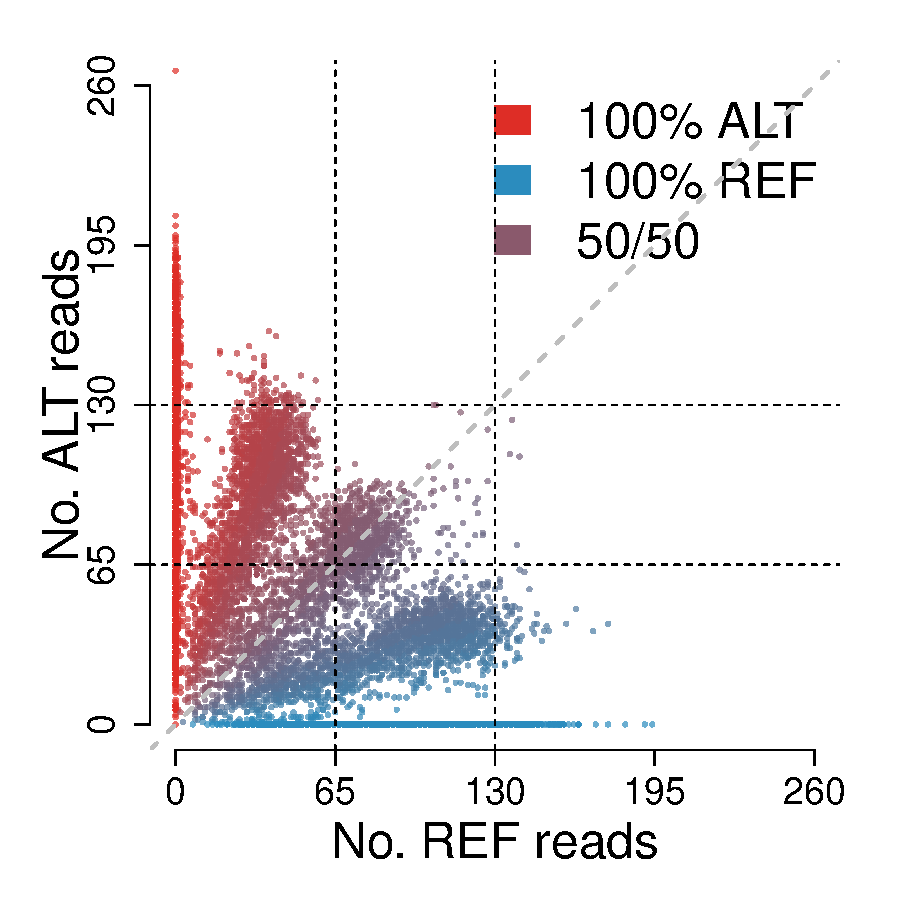
\includegraphics[width=0.35\textwidth]{altVsRef.pdf}}
  %\subfloat[][]{\includegraphics[width=0.65\textwidth]{hap_viterbi_hap1.pdf}}
  %\subfloat[][]{\includegraphics[width=0.65\textwidth]{hap_viterbi_hap2.pdf}}
\sbox{\measurebox}{%
  \begin{minipage}[b]{.38\textwidth}
  \subfloat
    []
    {\label{fig:figA}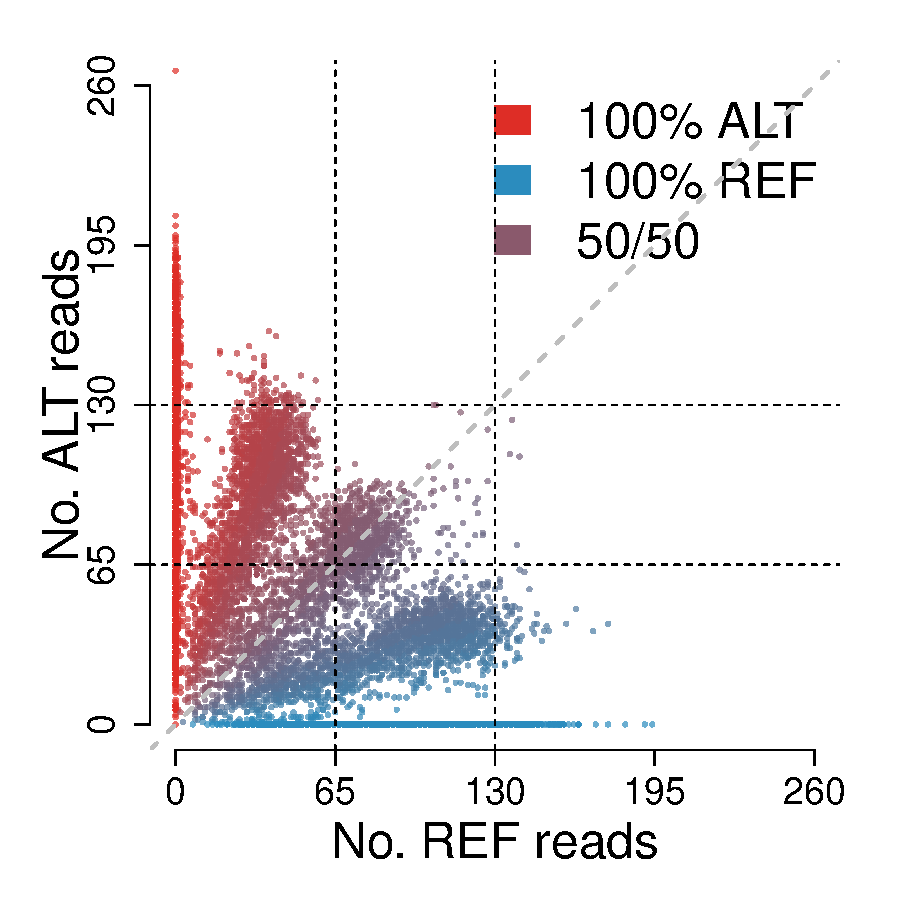
\includegraphics[width=\textwidth]{altVsRef.pdf}}
  \end{minipage}}
\usebox{\measurebox}%\qquad
\begin{minipage}[b][\ht\measurebox][s]{.62\textwidth}
%\centering
\subfloat
  []
  {\label{fig:figB}\includegraphics[width=\textwidth]{hap_viterbi_hap1.pdf}}\\
%\vfill
\subfloat
  []
  {\label{fig:figC}\includegraphics[width=\textwidth]{hap_viterbi_hap2.pdf}}
\end{minipage}

\end{figure}
\end{document}

